\documentclass{article}

\usepackage[spanish,es-tabla]{babel}
\usepackage[utf8]{inputenc}
\usepackage[T1]{fontenc}

\usepackage{times}        % fuente tipo paper
\usepackage{geometry}
\geometry{margin=2cm}

\usepackage{setspace}
\setlength{\columnsep}{0.7cm}  % espacio entre columnas

\usepackage{graphicx}
\usepackage{amsmath}
\usepackage{amssymb}

\usepackage{float}          % permite el especificador [H]
\usepackage{placeins}       % permite \FloatBarrier

\usepackage{booktabs}

\usepackage[numbers]{natbib}

\usepackage{hyperref}
\hypersetup{
    colorlinks=true,
    citecolor=blue,
    linkcolor=blue,
    urlcolor=blue
}
\title{Valoracion de la opcion de CAN-USD}
\author{
    Oscar Díaz\\
    Felipe Murillo\\
    \textit{Asesor: Ferddy H. Marín}
}
\date{}

\begin{document}

\maketitle

\section*{Resumen}
Este trabajo evalúa empíricamente la modelación de la tasa de cambio del dólar canadiense frente al dólar estadounidense (DEXCAUS) mediante un Movimiento Browniano Geométrico (MBG) y valora opciones de compra europeas sobre dicho subyacente. A partir de 250 observaciones diarias comprendidas entre noviembre de 2025 y noviembre de 2026, se verificaron los supuestos del modelo sobre los retornos logarítmicos: las pruebas de Jarque-Bera, Kolmogorov-Smirnov y Lilliefors no rechazaron la normalidad, la prueba de Dickey-Fuller Aumentada confirmó la estacionariedad de las perturbaciones, y los tests ARCH de Engle y Ljung-Box descartaron heterocedasticidad condicional; la dimensión fractal y el exponente de Hurst corroboraron la ausencia de memoria de largo plazo relevante. Estimados los parámetros del proceso, el pronóstico sobre la muestra cumplió el criterio de un error porcentual absoluto medio (MAPE) inferior al $5\%$. Con la volatilidad histórica estimada se valoraron veinte opciones Call europeas, combinando cuatro vencimientos con cinco precios de ejercicio cada uno, mediante la fórmula cerrada de Black-Scholes, simulación de Monte Carlo, el árbol binomial de Cox-Ross-Rubinstein y diferencias finitas explícitas. Tomando Black-Scholes como referencia, los tres métodos numéricos reprodujeron sus precios con errores relativos reducidos y revelaron un compromiso claro entre exactitud y costo computacional: las diferencias finitas alcanzaron la mayor precisión y Monte Carlo el menor tiempo de cómputo. Los resultados confirman la pertinencia del MBG y del modelo de Black-Scholes como herramientas cuantitativas para el análisis de riesgo en el mercado de divisas.

\vspace{0.5em}
\noindent\textbf{Palabras clave:} Movimiento Browniano Geométrico; valoración de opciones; opciones Call europeas; modelo de Black-Scholes; simulación de Monte Carlo; árbol binomial; diferencias finitas; tasa de cambio CAD/USD.

\section*{Introducción}
La modelación de activos financieros y la valoración de instrumentos derivados constituyen herramientas fundamentales para la toma de decisiones en los mercados financieros y en el sector real de la economía. Su importancia radica en que las empresas, independientemente de su actividad económica, se encuentran expuestas a variaciones en variables financieras como las tasas de interés, los precios de los activos, las tasas de cambio y la volatilidad de los mercados. Estas cambios pueden afectar directamente sus costos de financiación, sus inversiones, sus flujos de caja y su rentabilidad. En este sentido, contar con modelos que permitan describir el comportamiento de los activos financieros resulta esencial para cuantificar riesgos, estimar escenarios futuros y diseñar estrategias que contribuyan a una adecuada gestión financiera.

En particular, la valoración de instrumentos derivados, como las opciones financieras, desempeña un papel importante en la administración de la incertidumbre. Las opciones otorgan a su comprador el derecho, pero no la obligación, de comprar o vender un activo a un precio previamente establecido durante un periodo determinado. Esto permite que las empresas y los inversionistas implementen estrategias de cobertura frente a movimientos desfavorables de los precios, protejan sus inversiones y gestionen su exposición al riesgo, sin renunciar necesariamente a la posibilidad de beneficiarse de movimientos favorables del mercado. Por tanto, su valoración adecuada es relevante no solo para los participantes del mercado financiero, sino también para las organizaciones del sector real que buscan reducir la incertidumbre asociada a sus operaciones e inversiones.

Para estudiar la dinámica de los activos financieros, uno de los modelos estocásticos ampliamente utilizados es el Movimiento Browniano Geométrico, el cual supone que los rendimientos logarítmicos del activo siguen una distribución normal y que sus incrementos son independientes y estacionarios. Este modelo permite representar la evolución de los precios mediante dos parámetros principales, la tasa de rendimiento esperado y la volatilidad. Además, constituye uno de los fundamentos matemáticos del modelo de Black-Scholes, utilizado para obtener el precio teórico de opciones europeas. Sin embargo, dado que se trata de una representación idealizada del comportamiento de los mercados, es necesario evaluar empíricamente sus supuestos antes de utilizarlo para realizar pronósticos o valorar instrumentos financieros.

De esta manera, se busca integrar la modelación estocástica de activos financieros con las técnicas de valoración de instrumentos derivados, examinando tanto la capacidad descriptiva y predictiva del modelo como las diferencias numéricas entre los métodos de valoración. Con ello, se pretende comprender la utilidad de estas herramientas para el análisis financiero, la cuantificación de la incertidumbre y la toma de decisiones relacionadas con la gestión del riesgo.

\section*{Preliminares matemáticos}

\textbf{Movimiento browniano}: El movimiento browniano es un proceso estocástico de tiempo continuo y espacio de estados real, que permite modelar fenómenos cuya evolución presenta fluctuaciones aleatorias~\cite{einstein1905brownian, siegrist2022brownian}. Se caracteriza porque sus incrementos son independientes, estacionarios y tienen una distribución normal, además de poseer trayectorias continuas en la mayoria de los casos.
\\
\\
\textbf{Movimiento browniano Geometrico}: El movimiento browniano geométrico (MBG) es el proceso estocástico en tiempo continuo que fundamenta la mayoría de los modelos clásicos de precios de activos~\cite{metricgate2025mbg}, dinámica de poblaciones y crecimiento multiplicativo aleatorio. A diferencia del movimiento browniano estándar, el MBG garantiza que los valores permanezcan estrictamente positivos y genera variables con distribución log-normal, propiedades que describen diversos fenómenos reales. Destaca fundamentalmente como el modelo subyacente de precios de activos en el marco de la valoración de opciones de Black-Scholes. Formalmente, el precio del activo $S_t$ bajo el MBG satisface la ecuación diferencial estocástica

\begin{equation}
dS_t=\mu\,S_t\,dt+\sigma\,S_t\,dW_t,
\label{eq:mbg}
\end{equation}

donde $\mu$ es la tasa de rendimiento esperado, $\sigma$ la volatilidad y $W_t$ un movimiento browniano estándar~\cite{metricgate2025mbg}.

Para que una serie de datos pueda modelarse adecuadamente mediante el MBG, sus retornos deben satisfacer un conjunto de supuestos derivados de la propia definición del proceso~\cite{marin2025blackscholes}. El primero es la \textit{normalidad} de los retornos logarítmicos, consecuencia directa de que los incrementos del movimiento browniano se distribuyen de forma gaussiana; su verificación se apoya en pruebas de bondad de ajuste como Jarque-Bera, Kolmogorov-Smirnov y Lilliefors. El segundo es la \textit{independencia y estacionariedad} de los incrementos: el MBG supone que los retornos no presentan memoria ni tendencias deterministas, lo que se traduce en que las perturbaciones del proceso deben constituir una serie estacionaria, condición que se contrasta con pruebas de raíz unitaria como la de Dickey-Fuller Aumentada. El tercero es la \textit{homocedasticidad} o volatilidad constante en el tiempo: dado que $\sigma$ es un parámetro fijo en la ecuación~\eqref{eq:mbg}, la varianza de los retornos no debe depender del instante ni exhibir agrupamientos de volatilidad. La presencia de estos agrupamientos indicaría estructuras de heterocedasticidad condicional de tipo ARCH o GARCH~\cite{engle1982arch, bollerslev1986garch}, incompatibles con el supuesto de volatilidad constante; su ausencia se verifica mediante el test ARCH de Engle y la prueba de Ljung-Box aplicada sobre los residuos al cuadrado.

Como diagnóstico complementario de la independencia de los incrementos, el carácter browniano de la serie puede caracterizarse a través de su geometría mediante la dimensión fractal (DF) y el exponente de Hurst (EH)~\cite{mandelbrot1983fractal, hurst1951longterm}. El exponente de Hurst mide la memoria de largo plazo de la serie: un valor cercano a $0{,}5$ indica incrementos independientes propios de un proceso browniano, mientras que valores alejados señalan persistencia ($\text{EH}>0{,}5$) o antipersistencia ($\text{EH}<0{,}5$). La dimensión fractal cuantifica la irregularidad de la trayectoria y, para un movimiento browniano estándar, se espera un valor cercano a $1{,}5$. Ambos indicadores están ligados por la relación $\text{DF}+\text{EH}\approx 2$, de modo que su suma constituye una comprobación conjunta de que la serie se comporta como una trayectoria browniana sin memoria de largo plazo relevante~\cite{mandelbrot1983fractal}.
\\
\\
\textbf{Modelo de Black-Scholes}: El modelo de Black-Scholes, desarrollado por Fischer Black y Myron Scholes (1973)~\cite{blackscholes1973}, constituye uno de los principales modelos matemáticos utilizados para la valoración de opciones financieras. Este modelo describe la evolución del precio de un activo financiero mediante un movimiento browniano geométrico, incorporando parámetros como la tasa de crecimiento esperada y la volatilidad. A partir de este planteamiento, establece una formulación matemática para determinar el precio teórico de opciones europeas, bajo determinados supuestos sobre el comportamiento del mercado y la ausencia de oportunidades de arbitraje. Para una opción de compra (call) europea, la solución analítica cerrada del modelo es~\cite{blackscholes1973, marin2025blackscholes}

\begin{equation}
C=S_0\,N(d_1)-K\,e^{-rT}\,N(d_2),
\qquad
d_1=\frac{\ln\!\left(\dfrac{S_0}{K}\right)+\left(r+\tfrac{1}{2}\sigma^2\right)T}{\sigma\sqrt{T}},
\qquad
d_2=d_1-\sigma\sqrt{T},
\label{eq:bs}
\end{equation}

donde $S_0$ es el precio spot del subyacente, $K$ el precio de ejercicio, $r$ la tasa libre de riesgo, $T$ el tiempo de maduración, $\sigma$ la volatilidad y $N(\cdot)$ la función de distribución acumulada de una variable normal estándar. Los términos $d_1$ y $d_2$ miden, en unidades de volatilidad, la posición del precio esperado del subyacente respecto al precio de ejercicio.
\\
\\
\textbf{Simulación Monte Carlo}: La Simulación de Montecarlo es una técnica matemática que se utiliza para estimar los posibles resultados de un evento incierto\cite{ibm_montecarlo}.A diferencia de un modelo de pronóstico normal, la simulación de Montecarlo predice un conjunto de resultados basados en un rango estimado de valores frente a un conjunto de valores de entrada fijos. En otras palabras, una simulación de Montecarlo construye un modelo de posibles resultados aprovechando una distribución de probabilidad, como una distribución uniforme o normal, para cualquier variable que tenga incertidumbre inherente. Aplicada a la valoración de opciones, estima el precio como el valor esperado del pago descontado bajo la medida de riesgo neutral, aproximando dicha esperanza por el promedio sobre $M$ trayectorias simuladas del subyacente~\cite{marin2025metodos}. En lugar de la discretización de Euler, el precio terminal se genera con la solución exacta del MBG,

\begin{equation}
S_T^{(i)}=S_0\,\exp\!\left[\left(r-\tfrac{1}{2}\sigma^2\right)T+\sigma\sqrt{T}\,Z^{(i)}\right],
\qquad Z^{(i)}\sim N(0,1),
\label{eq:mc_st}
\end{equation}

lo que elimina el error de discretización al depender el pago europeo únicamente de $S_T$. Adicionalmente puede aplicarse la técnica de reducción de varianza de variables antitéticas, que para cada normal $Z^{(i)}$ evalúa también su reflejo $-Z^{(i)}$ y promedia ambos pagos. El estimador del precio es

\begin{equation}
\widehat{C}=e^{-rT}\,\frac{1}{M}\sum_{i=1}^{M}
\frac{\max\!\left(S_T^{(i,+)}-K,\,0\right)+\max\!\left(S_T^{(i,-)}-K,\,0\right)}{2},
\label{eq:mc_precio}
\end{equation}

donde $S_T^{(i,\pm)}$ es el precio terminal generado con $\pm Z^{(i)}$, $M$ el número de pares de trayectorias y los demás símbolos conservan el significado de la ecuación~\eqref{eq:bs}. Junto al precio se reporta el error estándar de la estimación, $w/\sqrt{M}$, siendo $w$ la desviación estándar muestral de los pagos descontados.
\\
\\
\textbf{Árboles Binomiales}:Los árboles binomiales son un método numérico que permite representar la evolución de una variable a lo largo del tiempo mediante una estructura de posibles escenarios~\cite{coxrossrubinstein1979}. Este método divide el tiempo en intervalos discretos y considera que, en cada intervalo, el valor de la variable puede tomar dos direcciones posibles: aumentar o disminuir. A partir de estas posibilidades se construye una estructura en forma de árbol que muestra las diferentes trayectorias que puede seguir el proceso. Cada transición está asociada a una probabilidad, lo que permite estudiar la distribución de los posibles valores futuros. Este enfoque facilita la aproximación de procesos estocásticos continuos mediante modelos discretos y permite analizar su comportamiento a través de un número finito de escenarios. En la formulación de Cox-Ross-Rubinstein, el horizonte se discretiza en $N$ pasos de longitud $\Delta t=T/N$, y los factores de salto junto con la probabilidad de riesgo neutral se fijan como~\cite{coxrossrubinstein1979, marin2025metodos}

\begin{equation}
u=e^{\sigma\sqrt{\Delta t}},\qquad
d=\frac{1}{u},\qquad
p=\frac{e^{r\,\Delta t}-d}{u-d}.
\label{eq:crr_param}
\end{equation}

Esta probabilidad $p$ iguala el valor esperado del subyacente a $S_0e^{r\Delta t}$. Partiendo del pago en el vencimiento, $f_{N,j}=\max(S_{N,j}-K,0)$, la opción se valora hacia atrás descontando en cada nodo el valor esperado de riesgo neutral, de modo que el valor en un nodo interior satisface

\begin{equation}
f_{i,j}=e^{-r\,\Delta t}\left[p\,f_{i+1,j+1}+(1-p)\,f_{i+1,j}\right],
\label{eq:crr_induccion}
\end{equation}

donde $f_{i,j}$ es el valor de la opción en el nodo $(i,j)$, $p$ la probabilidad de riesgo neutral de un salto al alza y $r$ la tasa libre de riesgo.
\\
\\
\textbf{Diferencias Finitas Explícitas}: Las diferencias finitas explícitas son un método numérico utilizado para aproximar soluciones de ecuaciones diferenciales mediante la discretización de las variables independientes, como el tiempo y el espacio~\cite{gurevich2008numerical}. El método consiste en sustituir las derivadas por aproximaciones algebraicas basadas en los valores de la función en puntos cercanos de una malla. Se caracteriza porque permite calcular directamente el valor aproximado de la solución en un instante posterior utilizando los valores conocidos del instante actual, sin necesidad de resolver un sistema de ecuaciones en cada paso. Este procedimiento facilita la implementación computacional y permite estudiar la evolución de diferentes fenómenos mediante aproximaciones sucesivas. Sin embargo, la estabilidad y precisión del método dependen de la elección de los pasos de discretización, por lo que es necesario establecer condiciones que eviten la propagación de errores numéricos. Aplicado a la valoración de opciones, el método resuelve numéricamente la ecuación en derivadas parciales de Black-Scholes-Merton~\cite{gurevich2008numerical, marin2025metodos},

\begin{equation}
\frac{\partial f}{\partial t}+r\,S\,\frac{\partial f}{\partial S}+\frac{1}{2}\sigma^2 S^2\,\frac{\partial^2 f}{\partial S^2}=r\,f,
\label{eq:bsm_pde}
\end{equation}

donde $f=f(t,S)$ es el valor de la opción, $S$ el precio del subyacente, $t$ el tiempo, y $r$ y $\sigma$ la tasa libre de riesgo y la volatilidad. Mediante el cambio de variable $x=\ln S$ y el tiempo al vencimiento $\tau=T-t$, la ecuación~\eqref{eq:bsm_pde} se transforma en una ecuación de coeficientes constantes,

\begin{equation}
\frac{\partial V}{\partial \tau}=\frac{1}{2}\sigma^2\,\frac{\partial^2 V}{\partial x^2}
+\left(r-\tfrac{1}{2}\sigma^2\right)\frac{\partial V}{\partial x}-r\,V,
\label{eq:bsm_logprecio}
\end{equation}

con $V(\tau,x)=f(t,S)$. Al discretizar con pasos $\Delta x$ y $\Delta\tau$, el valor en cada nodo se obtiene explícitamente como

\begin{equation}
V_{j}^{\,k+1}=a\,V_{j-1}^{\,k}+b\,V_{j}^{\,k}+c\,V_{j+1}^{\,k},
\label{eq:fd_esquema}
\end{equation}
\begin{equation}
a=\Delta\tau\!\left(\frac{\sigma^2}{2\,\Delta x^2}-\frac{r-\tfrac12\sigma^2}{2\,\Delta x}\right),\quad
b=1-\Delta\tau\!\left(\frac{\sigma^2}{\Delta x^2}+r\right),\quad
c=\Delta\tau\!\left(\frac{\sigma^2}{2\,\Delta x^2}+\frac{r-\tfrac12\sigma^2}{2\,\Delta x}\right).
\label{eq:fd_coef}
\end{equation}

La estabilidad del esquema explícito requiere que el paso temporal respete la condición $\Delta\tau\le \Delta x^2/\sigma^2$, que garantiza coeficientes no negativos.

\section*{Metodología}
La metodología se organiza en cuatro etapas sucesivas. Primero se describe el conjunto de datos y su comportamiento estadístico básico. A continuación se verifica, mediante indicadores y pruebas estadísticas, que la serie satisface los supuestos del MBG. Verificados esos supuestos, se estiman los parámetros del modelo y se evalúa su capacidad predictiva sobre la muestra. Finalmente, con los parámetros calibrados se valoran opciones Call europeas por cuatro métodos y se comparan sus resultados.

\subsection*{Descripción de los datos}
Para el desarrollo de este trabajo, se utilizó un conjunto de datos consultados del Banco de la Reserva Federal de Saint Louis, ubicado en Missouri, Estados Unidos\footnote{Datos disponibles para su descarga en \url{https://fred.stlouisfed.org/}.}, que reportaba la tasa del activo subyacente (DEXCAUS o \(S_t\)) desde noviembre del 2025 hasta noviembre del 2026. Como se puede visualizar toda la serie en la Figura \ref{fig:plotSt}, el archivo contiene 261 registros en ese periodo, de los cuales 250 corresponden a cotizaciones efectivas y los 11 restantes a días festivos o no hábiles en los mercados que se descartan del análisis. El estudio trabaja, por tanto, sobre 250 observaciones válidas, por encima del mínimo exigido. La serie presenta fases claramente diferenciadas: entre noviembre de 2025 y principios de 2026 se observa un descenso desde niveles cercanos a 1,41 hasta un mínimo de aproximadamente 1,3518 en febrero de 2026. Posteriormente, la serie experimenta una recuperación con una fase de alta volatilidad y estabilización, alcanzando máximos locales alrededor de 1,4237 a mediados de año (junio-julio) y un pico superior cercano a 1,4273 en octubre de 2026. Estos movimientos son consistentes con factores documentados externamente, como las tensiones comerciales, las decisiones de política monetaria y los cambios en la confianza del mercado.

\begin{figure}[H]
    \centering
    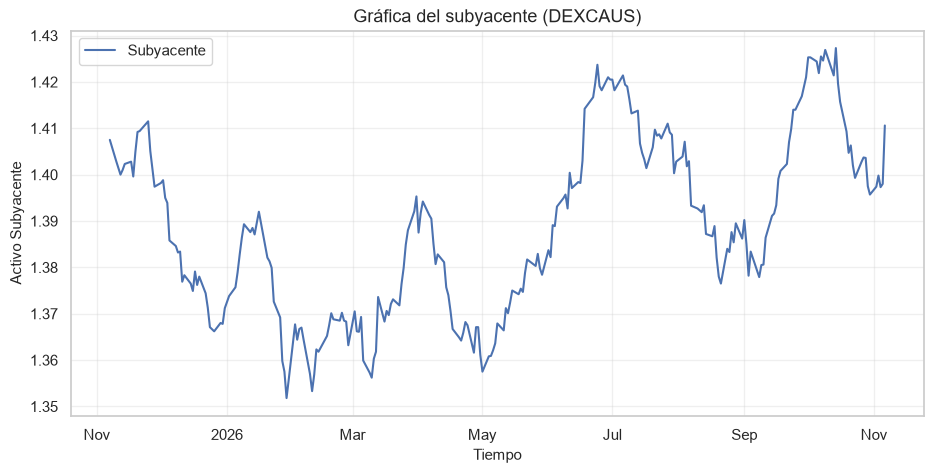
\includegraphics[width=1\textwidth]{images/plotSt.png}
    \caption{Evolución temporal de la serie del activo subyacente (DEXCAUS) entre noviembre de 2025 y noviembre de 2026.}
    \label{fig:plotSt}
\end{figure}

El comportamiento numérico de la serie se detalla de forma integral en la Tabla \ref{tab:estadisticas_subyacente}. Los estadísticos descriptivos reflejan una alta concentración de las observaciones en torno a su valor central y una baja variabilidad, cuya distribución empírica se complementa con el histograma de la Figura \ref{fig:hist_subyacente}. La Figura \ref{fig:pacf_subyacente} evidencia, por su parte, la estructura de dependencia de un único retardo para cada $S_t$.

\begin{table}[H]
\centering
\scriptsize
\resizebox{\textwidth}{!}{
\begin{tabular}{lrrrrrrrrr}
\hline
\textbf{} & \textbf{Mínimo} & \textbf{Máximo} & \textbf{Media} & \textbf{Mediana} & \textbf{Moda} & \textbf{Varianza} & \textbf{Desv. estándar} & \textbf{Curtosis} & \textbf{Asimetría} \\
\hline
\textbf{Subyacente} & 1.351800 & 1.427300 & 1.388349 & 1.387150 & 1.367100 & 0.000359 & 0.018949 & 2.033949 & 0.195183 \\
\hline
\end{tabular}
}
\caption{Estadísticas descriptivas del activo subyacente.}
\label{tab:estadisticas_subyacente}
\end{table}

\begin{figure}[H]
    \centering
    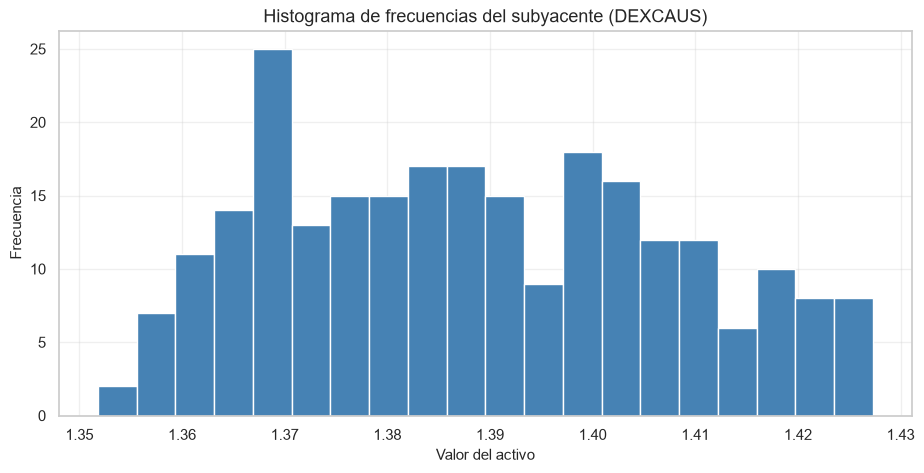
\includegraphics[width=1\textwidth]{images/histSt.png}
    \caption{Histograma de frecuencias y distribución empírica del activo subyacente (DEXCAUS).}
    \label{fig:hist_subyacente}
\end{figure}

\begin{figure}[H]
    \centering
    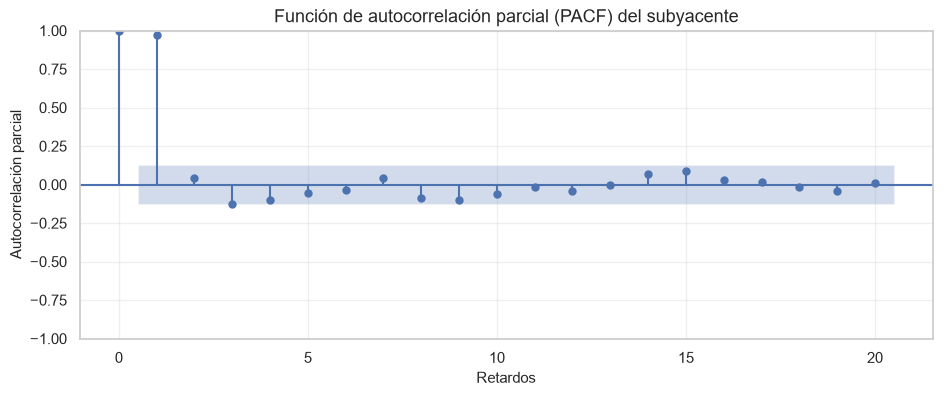
\includegraphics[width=1\textwidth]{images/pacfSt.png}
    \caption{Función de autocorrelación parcial (PACF) del activo subyacente.}
    \label{fig:pacf_subyacente}
\end{figure}

Como medida complementaria de la estructura de dependencia de la serie, se estimaron la dimensión fractal (DF) y el exponente de Hurst (EH), cuyos resultados se reportan en la Tabla \ref{tab:fractal_hurst}. Como se explicó en los Preliminares, estos indicadores caracterizan geométricamente el carácter browniano de la serie: para un movimiento browniano estándar se espera una dimensión fractal cercana a $1{,}5$, un exponente de Hurst próximo a $0{,}5$ (indicativo de incrementos independientes, sin memoria de largo plazo) y una suma $\text{DF}+\text{EH}\approx 2$. El exponente estimado, $\text{EH}=0{,}6091$, se ubica cerca de $0{,}5$ y descarta una persistencia marcada en los incrementos, mientras que la suma obtenida, $\text{DF}+\text{EH}=1{,}7599$, no se aleja sustancialmente del valor de referencia. En conjunto, estos indicadores respaldan que la serie no exhibe una memoria de largo plazo relevante y resulta una opción adecuada para ser modelada mediante un MBG, en coherencia con los supuestos de independencia de los incrementos del proceso.

\begin{table}[H]
\centering
\begin{tabular}{lcc}
\hline
Indicador & Valor & Desv. estándar \\
\hline
Dimensión fractal (DF)   & 1.150759 & 0.017872 \\
Exponente de Hurst (EH)  & 0.609134 & 0.008589 \\
DF + EH                  & 1.759893 & — \\
\hline
\end{tabular}
\caption{Dimensión fractal y exponente de Hurst de la serie del subyacente. Valores de referencia para un movimiento browniano estándar: $\text{DF}\approx 1{,}5$, $\text{EH}\approx 0{,}5$ y $\text{DF}+\text{EH}\approx 2$.}
\label{tab:fractal_hurst}
\end{table}

\subsection*{Indicadores y pruebas estadísticas}
Como se expuso en los Preliminares, para afirmar que la serie del tipo de cambio CAD/USD puede modelarse como un MBG es necesario verificar que sus retornos cumplen tres condiciones: normalidad, estacionariedad de las innovaciones y varianza constante (homocedasticidad). Con ese fin se trabajó sobre los retornos logarítmicos diarios y sobre las perturbaciones estandarizadas $E_t$, aplicando a un nivel de significancia del $5\%$ pruebas de normalidad (Jarque-Bera, Kolmogorov-Smirnov y Lilliefors), de estacionariedad (Dickey-Fuller Aumentada) y de homocedasticidad (ARCH de Engle y Ljung-Box). Se examina cada condición en ese orden.

Comenzando por la normalidad de los retornos, las pruebas de Jarque-Bera, Kolmogorov-Smirnov y Lilliefors no condujeron al rechazo de la hipótesis nula, tal como se detalla en la Tabla \ref{tab:normalidad}. 

Este comportamiento también se respalda gráficamente: el histograma de los retornos (Figura \ref{fig:hist_retornos}) muestra una distribución simétrica que exhibe un buen acoplamiento con la curva normal teórica ($\mu = 0{,}00001$, $\sigma = 0{,}00283$). Asimismo, el diagrama de caja y el gráfico Q-Q (Figura \ref{fig:QQ-Box}) confirman la alineación general de la mayoría de las observaciones con los cuantiles teóricos, evidenciando únicamente ligeras desviaciones y algunos valores atípicos (outliers) en las colas. Dado que ninguna de las pruebas formales rechaza la normalidad y la evidencia visual respalda el ajuste global, se concluye que no existe evidencia suficiente para abandonar el supuesto de normalidad de los retornos, el cual constituye una condición necesaria del MBG.

\begin{table}[H]
\centering
\begin{tabular}{lccc}
\hline
Prueba & Estadístico & Valor-p & h (1 = rechaza normalidad) \\
\hline
Jarque-Bera & 1.966114 & 0.374166 & 0 \\
Kolmogorov-Smirnov & 0.041930 & 0.757449 & 0 \\
Lilliefors & 0.041930 & 0.424762 & 0 \\
\hline
\end{tabular}
\caption{Pruebas de normalidad de los retornos logarítmicos diarios.}
\label{tab:normalidad}
\end{table}

\begin{figure}[H]
    \centering
    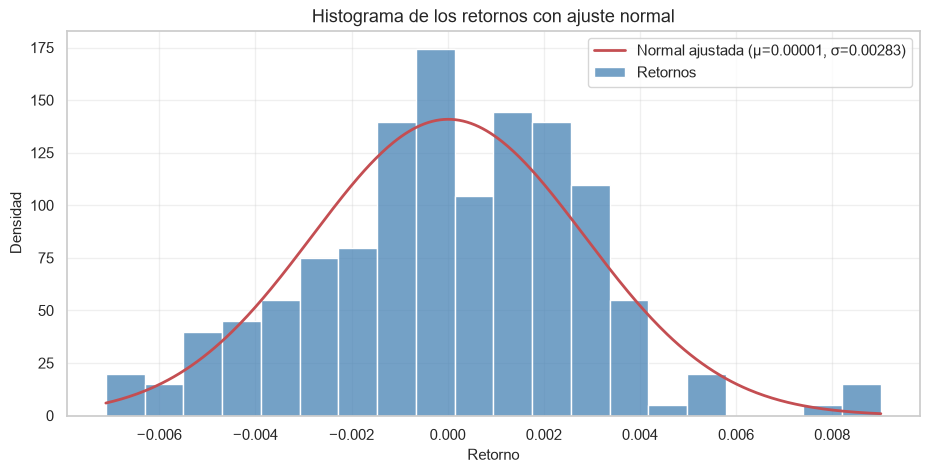
\includegraphics[width=0.85\linewidth]{images/histRt.png}
    \caption{Histograma de los retornos logarítmicos diarios con ajuste de distribución normal.}
    \label{fig:hist_retornos}
\end{figure}

\begin{figure}[H]
    \centering
    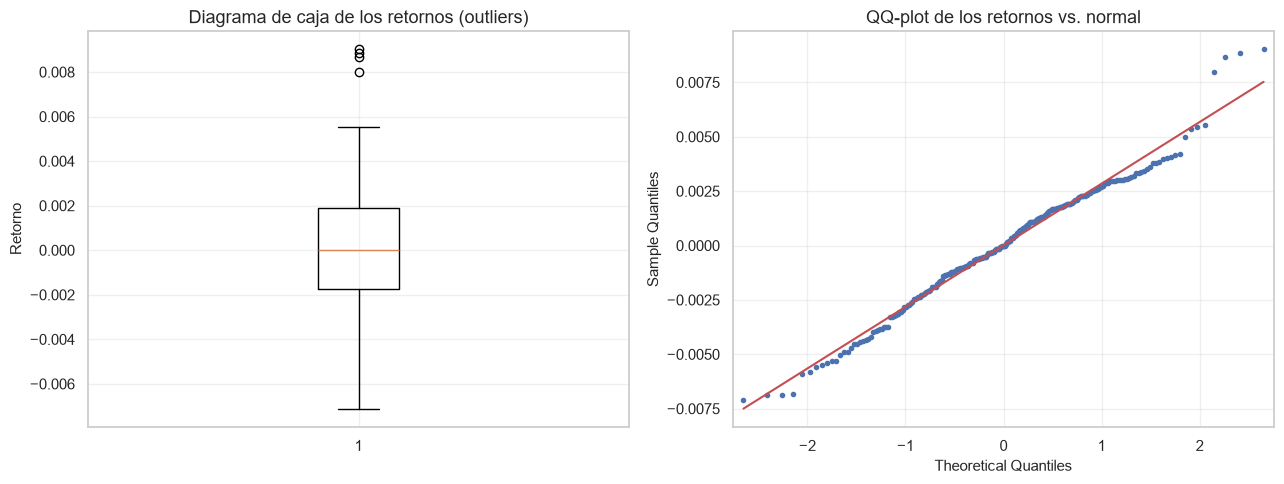
\includegraphics[width=1\linewidth]{images/QQ-Box_plotRt.png}
    \caption{Diagrama de caja (izquierda) y gráfico Q-Q (derecha) de los retornos logarítmicos frente a la distribución normal teórica.}
    \label{fig:QQ-Box}
\end{figure}

Respecto a la estacionariedad, la prueba de Dickey-Fuller Aumentada (sin constante y sin rezagos) aplicada a las perturbaciones estandarizadas condujo al rechazo de la hipótesis nula de raíz unitaria al nivel de significancia del $5\%$, según se detalla en la Tabla \ref{tab:adf}. Este resultado confirma que las innovaciones constituyen un proceso estacionario, cumpliendo así con la estructura teórica exigida por el modelo. Asimismo, esta conclusión se respalda visualmente en la Figura \ref{fig:perturbaciones}, donde se observa que la serie oscila de manera estable alrededor de una media cero y mantiene una dispersión constante a lo largo del tiempo, sin evidenciar tendencias ni cambios estructurales.

\begin{table}[H]
\centering
\begin{tabular}{lcccc}
\hline
Prueba & h & Valor Crítico (5\%) & Estadístico & Valor-p \\
\hline
ADF & 1 & -1.942136 & -14.992976 & 0.000000 \\
\hline
\end{tabular}
\caption{Prueba de raíz unitaria Dickey-Fuller Aumentada (sin constante y sin rezagos) aplicada a las perturbaciones.}
\label{tab:adf}
\end{table}

\begin{figure}[H]
    \centering
    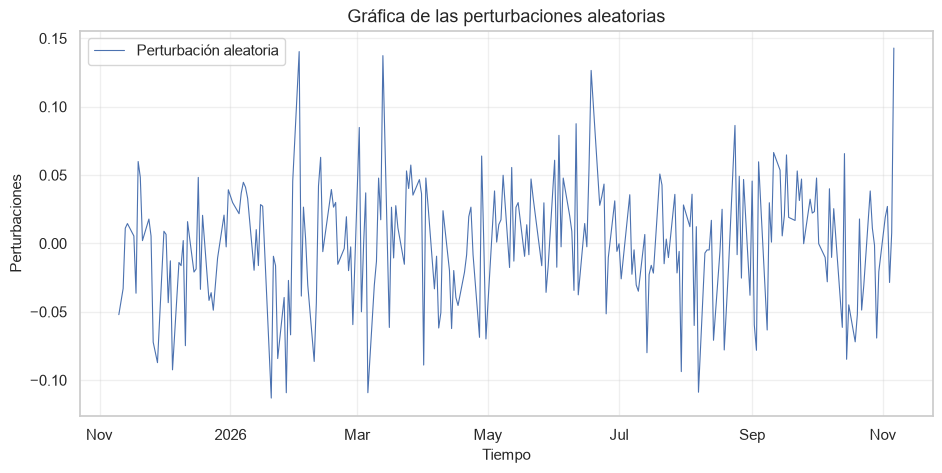
\includegraphics[width=1\linewidth]{images/plotEt.png}
    \caption{Serie temporal de las perturbaciones estandarizadas $E_t$.}
    \label{fig:perturbaciones}
\end{figure}

Queda por verificar la tercera condición, la varianza constante. El test ARCH de Engle con cinco rezagos no condujo al rechazo de la hipótesis nula al nivel de significancia del $5\%$, según se reporta en la Tabla \ref{tab:arch}, por lo que se descarta la presencia de efectos ARCH en las perturbaciones. La prueba de Ljung-Box aplicada sobre los residuos al cuadrado con cinco rezagos tampoco evidenció el rechazo de su hipótesis nula, tal como se muestra en la Tabla \ref{tab:ljungbox}. Esto permite descartar autocorrelación significativa en la varianza y, con ello, posibles efectos de tipo GARCH, confirmando así el supuesto de homocedasticidad condicional (varianza constante) requerido por la especificación del modelo.

\begin{table}[H]
\centering
\begin{tabular}{lcccc}
\hline
Prueba & h & Valor Crítico & Estadístico & Valor-p \\
\hline
ARCH (5 rezagos) & 0 & 11.070498 & 9.910051 & 0.077824 \\
\hline
\end{tabular}
\caption{Test ARCH de Engle con cinco rezagos sobre las perturbaciones.}
\label{tab:arch}
\end{table}

\begin{table}[H]
\centering
\begin{tabular}{lcccc}
\hline
Prueba & h & Valor Crítico & Estadístico & Valor-p \\
\hline
Ljung-Box (5 rezagos) & 0 & 11.070498 & 8.511854 & 0.130192 \\
\hline
\end{tabular}
\caption{Prueba de Ljung-Box sobre los residuos al cuadrado con cinco rezagos.}
\label{tab:ljungbox}
\end{table}

En conjunto, la aceptación de estos cuatro diagnósticos, normalidad aproximada de los retornos (Tabla \ref{tab:normalidad}), estacionariedad de las perturbaciones (Tabla \ref{tab:adf}), ausencia de efectos ARCH (Tabla \ref{tab:arch}) y ausencia de autocorrelación en la varianza (Tabla \ref{tab:ljungbox}), permite afirmar técnicamente que el fenómeno satisface los supuestos del MBG y que, por tanto, puede ser modelado bajo el marco de Black-Scholes.

\subsection*{Estimación de parámetros y pronóstico sobre la muestra}
Verificada la varianza constante, el paso siguiente es cuantificar su nivel. Como validación empírica previa a la estimación, se analizó la evolución temporal de la volatilidad acumulada del subyacente mediante una ventana de crecimiento expansivo, tal como se muestra en la Figura \ref{fig:volatilidad}. Aunque el modelo asume un valor de $\sigma$ constante, este gráfico permite observar cómo, tras una etapa inicial de mayor fluctuación propia de un tamaño de muestra reducido, la volatilidad se asienta hacia un nivel uniforme, lo que confirma que la estimación muestral deja de ser sensible a modificaciones marginales en la ventana temporal analizada.

\begin{figure}[H]
    \centering
    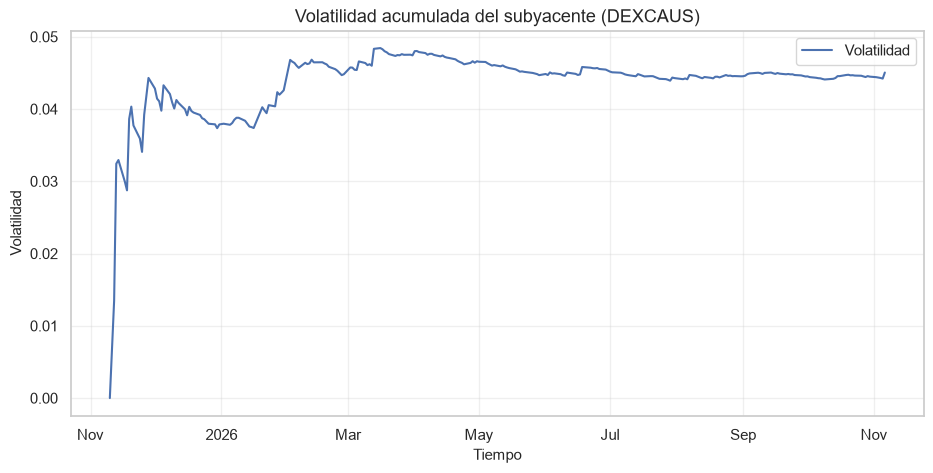
\includegraphics[width=1\linewidth]{images/volatility.png}
    \caption{Evolución de la volatilidad acumulada del subyacente (DEXCAUS) estimada mediante ventana expansiva.}
    \label{fig:volatilidad}
\end{figure}

Sobre esta base, la estimación de los parámetros del MBG ($\widehat{\mu}$ y $\widehat{\sigma}$) se realizó mediante dos enfoques complementarios detallados en la Tabla \ref{tab:parametros_mbg}: el primero corresponde al esquema basado en retornos simples bajo la discretización de Euler-Maruyama, mientras que el segundo emplea los log-retornos en coherencia con la solución exacta del proceso estocástico. 

\begin{table}[H]
\centering
\begin{tabular}{lcccc}
\hline
Método de estimación & $\widehat{\mu}$ & $\widehat{\sigma}$ & $\widehat{\mu}$ anualizada & $\widehat{\sigma}$ anualizada \\
\hline
Retornos simples (Euler-Maruyama) & 0.003237 & 0.045046 & — & — \\
Log-retornos (solución exacta)     & 0.003241 & 0.045045 & 0.32\% & 4.50\% \\
\hline
\end{tabular}
\caption{Estimación de los parámetros del MBG por dos vías complementarias.}
\label{tab:parametros_mbg}
\end{table}

Como se evidencia en la Tabla \ref{tab:parametros_mbg}, existe una coincidencia prácticamente exacta entre los resultados de ambas metodologías, lo que confirma la estabilidad numérica y la consistencia de la calibración. El valor estimado para la volatilidad ($\widehat{\sigma}$) coincide además con el nivel hacia el que se asienta la volatilidad acumulada de la Figura \ref{fig:volatilidad}. Queda así validado el uso de esta volatilidad histórica constante como insumo tanto para la generación de trayectorias de pronóstico como para la valoración de opciones.

Con estos parámetros se generaron tanto las trayectorias inducidas (Figura \ref{fig:pronostico_inducido}) como las simuladas (Figura \ref{fig:pronostico_simulado}) del MBG a partir del último dato observado, evaluando su desempeño predictivo mediante el error porcentual absoluto medio (MAPE). Los resultados evidencian un buen ajuste en ambos enfoques; además, se reporta la cobertura de las bandas de confianza construidas al $95\%$ alrededor de la trayectoria esperada, comprobando que el valor efectivo de la serie cae dentro del intervalo proyectado en la mayor parte del horizonte, tal como se resume en la Tabla \ref{tab:metricas_pronostico}.

\begin{figure}[H]
    \centering
    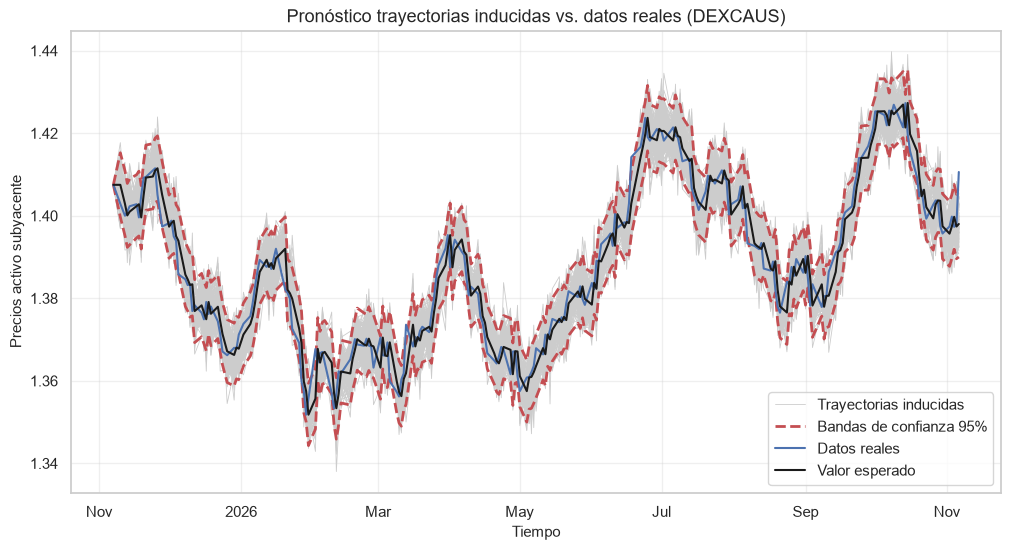
\includegraphics[width=1\linewidth]{images/pronosticoInducido.png}
    \caption{Pronóstico de trayectorias inducidas vs. datos reales.}
    \label{fig:pronostico_inducido}
\end{figure}

\begin{figure}[H]
    \centering
    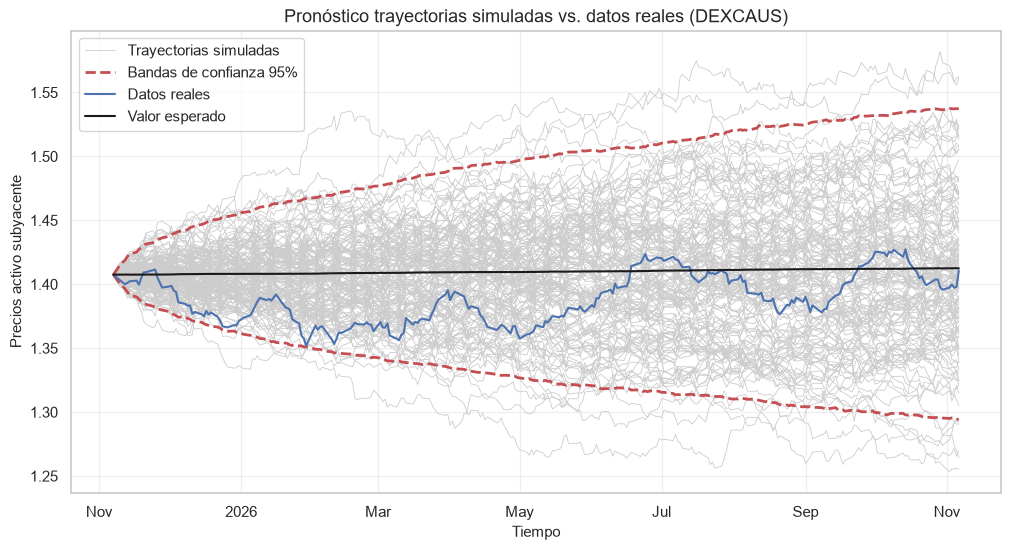
\includegraphics[width=1\linewidth]{images/pronosticoSimulado.png}
    \caption{Pronóstico de trayectorias simuladas vs. datos reales.}
    \label{fig:pronostico_simulado}
\end{figure}

\begin{table}[H]
\centering
\begin{tabular}{lcc}
\hline
Métrica & Trayectorias inducidas & Trayectorias simuladas \\
\hline
MAPE mínimo ($\%$) & 0.2725 & 0.6529 \\
MAPE promedio ($\%$) & 0.3170 & 2.9709 \\
MAPE máximo ($\%$) & 0.3643 & 10.7870 \\
Cobertura de las bandas al 95\% & 95.60\% (0.9560) & 100.00\% (1.0000) \\
\hline
\end{tabular}
\caption{Métricas de desempeño para las trayectorias inducidas y simuladas del MBG.}
\label{tab:metricas_pronostico}
\end{table}

\subsection*{Valoración de opciones Call europeas}
El pronóstico anterior proyecta la serie sobre su propio horizonte muestral para validar el ajuste del modelo. La valoración de opciones, en cambio, requiere proyectar el subyacente más allá del último dato observado: se pasa así de la simulación sobre la muestra a una simulación fuera de muestra, con la que se construyen los precios de ejercicio de los contratos. Esta valoración se realizó con una tasa libre de riesgo de $r=0{,}05$, sin dividendos, tomando como precio spot el último dato de la serie, $S_0=1{,}4106$ CAD/USD, y empleando la volatilidad histórica estimada, $\widehat{\sigma}=0{,}045045$. A partir de estos insumos, el procedimiento de construcción de los contratos a valorar se organizó en las siguientes etapas.

En primer lugar, se fijaron cuatro fechas de maduración, $T\in\{1;\,\tfrac{1}{2};\,\tfrac{1}{3};\,\tfrac{1}{4}\}$ años, que representan horizontes de uno, seis, cuatro y tres meses. Para cada una de estas maduraciones se simularon $10\,000$ trayectorias fuera de muestra del MBG partiendo del precio spot $S_0$ bajo la medida de riesgo neutral. Al evaluar cada conjunto de trayectorias en su respectivo tiempo final $T$ se obtuvo la distribución simulada del precio terminal del subyacente, $S_T$, que por la propiedad de log-normalidad del MBG se concentra alrededor del valor spot y se dispersa más a medida que crece el horizonte~\cite{marin2025blackscholes}.

En segundo lugar, sobre cada distribución simulada de $S_T$ se calcularon los percentiles 10, 25, 50, 75 y 90, y cada uno de ellos se adoptó como un precio de ejercicio $K$. De esta forma, para cada maduración se definieron cinco precios de ejercicio que cubren de manera representativa el rango plausible del subyacente al vencimiento, desde opciones con $K$ por debajo del spot (percentiles inferiores) hasta opciones con $K$ por encima del spot (percentiles superiores). Al repetir este proceso para las cuatro maduraciones se generó un total de veinte combinaciones $(T,K)$. La Figura \ref{fig:precioStrike} ilustra, para cada $T$, la distribución simulada de $S_T$ junto con los cinco precios de ejercicio así obtenidos, y la Tabla \ref{tab:combinaciones_TK} reúne el conjunto completo de precios de ejercicio por maduración.

\begin{figure}[H]
    \centering
    \begin{tabular}{cc}
        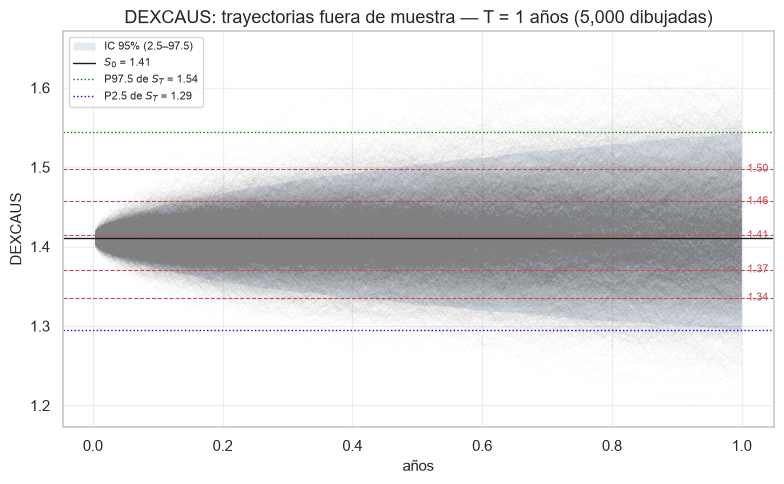
\includegraphics[width=0.47\textwidth]{images/simulacionPrecioStrike_T1.png} &
        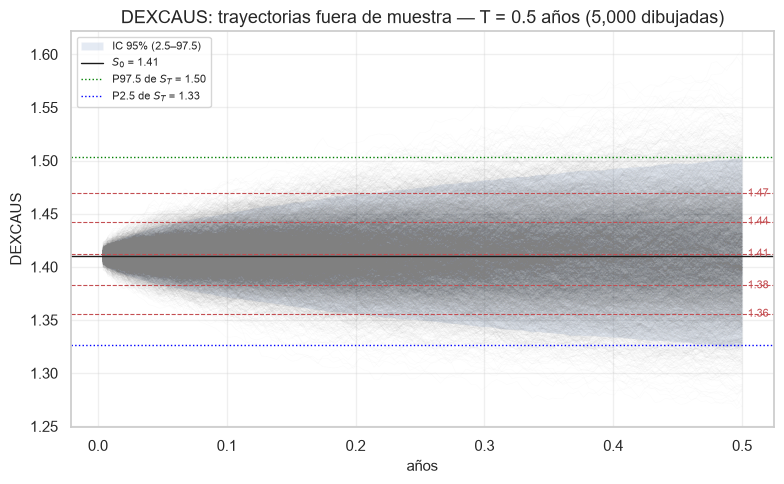
\includegraphics[width=0.47\textwidth]{images/simulacionPrecioStrike_T2.png} \\
        {\footnotesize (a) $T=1$ año} & {\footnotesize (b) $T=1/2$ año} \\[4pt]
        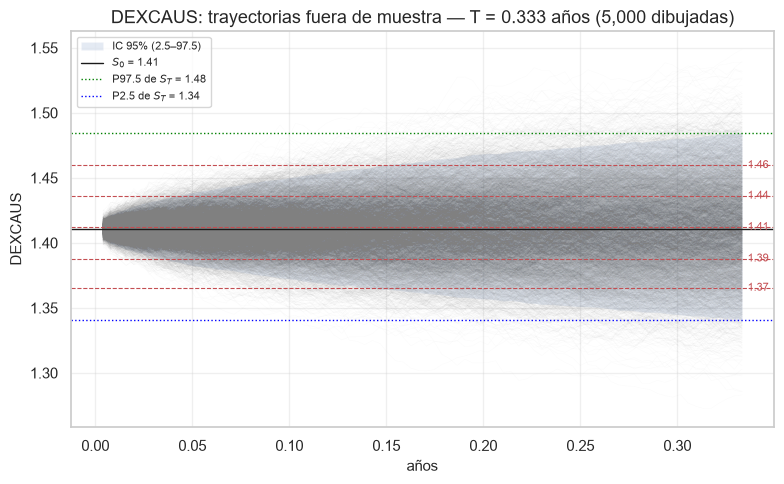
\includegraphics[width=0.47\textwidth]{images/simulacionPrecioStrike_T3.png} &
        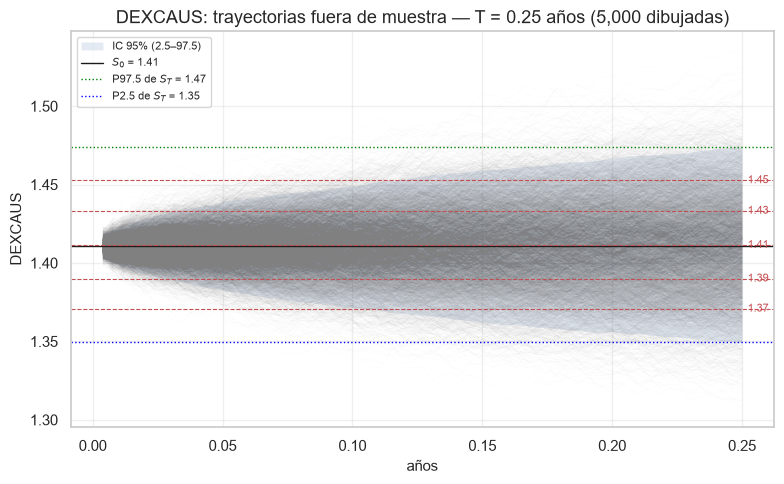
\includegraphics[width=0.47\textwidth]{images/simulacionPrecioStrike_T4.png} \\
        {\footnotesize (c) $T=1/3$ año} & {\footnotesize (d) $T=1/4$ año} \\
    \end{tabular}
    \caption{Distribución simulada del precio terminal del subyacente $S_T$ y precios de ejercicio $K$ obtenidos como los percentiles 10, 25, 50, 75 y 90 de dicha distribución, para cada una de las cuatro maduraciones consideradas.}
    \label{fig:precioStrike}
\end{figure}

\begin{table}[H]
\centering
\begin{tabular}{lccccc}
\hline
$T$ (años) & $P_{10}$ & $P_{25}$ & $P_{50}$ & $P_{75}$ & $P_{90}$ \\
\hline
$T=1$      & 1.335700 & 1.371100 & 1.414200 & 1.457000 & 1.497900 \\
$T=0.5$    & 1.355800 & 1.382500 & 1.412400 & 1.442600 & 1.469100 \\
$T=0.3333$ & 1.365400 & 1.387900 & 1.412100 & 1.436200 & 1.459700 \\
$T=0.25$   & 1.370800 & 1.390000 & 1.411400 & 1.433200 & 1.452700 \\
\hline
\end{tabular}
\caption{Precios de ejercicio $K$ definidos a partir de los percentiles 10, 25, 50, 75 y 90 de la distribución simulada de $S_T$ para cada maduración $T$.}
\label{tab:combinaciones_TK}
\end{table}

Definidas las veinte combinaciones $(T,K)$, cada opción europea de compra se valoró mediante cuatro métodos, cuyas fórmulas y fundamentos se expusieron en los Preliminares matemáticos y que aquí se aplican al problema concreto. El primero es la fórmula cerrada de Black-Scholes de la ecuación~\eqref{eq:bs}, que se adopta como valor de referencia por tratarse de la solución analítica exacta del modelo bajo los supuestos verificados para el subyacente.

El segundo método es la simulación de Monte Carlo. Siguiendo el esquema de las ecuaciones~\eqref{eq:mc_st} y~\eqref{eq:mc_precio}, el precio terminal se generó con la solución exacta del MBG y el precio de la opción se estimó como el promedio del pago descontado, aplicando además la técnica de variables antitéticas para reducir la varianza. Se emplearon $10\,000$ trayectorias.

El tercer método es el árbol binomial de Cox-Ross-Rubinstein, con los factores de salto y la probabilidad de riesgo neutral de la ecuación~\eqref{eq:crr_param} y la inducción hacia atrás de la ecuación~\eqref{eq:crr_induccion}. Se utilizaron $1\,000$ pasos.

El cuarto método es el de diferencias finitas explícitas, que resuelve la ecuación de Black-Scholes-Merton~\eqref{eq:bsm_pde} sobre su forma en log-precio~\eqref{eq:bsm_logprecio} mediante el esquema explícito de las ecuaciones~\eqref{eq:fd_esquema} y~\eqref{eq:fd_coef}. Se usaron trescientos nodos a cada lado del precio spot, de modo que $S_0$ coincide exactamente con un nodo de la malla, y el paso temporal se fijó respetando la condición de estabilidad $\Delta\tau\le \Delta x^2/\sigma^2$.

Para comparar los tres métodos numéricos con la referencia analítica se calculó, en cada combinación $(T,K)$, el error relativo porcentual respecto al valor de Black-Scholes,

\begin{equation}
\text{Error relativo}(\%)=
\frac{\left|P_{\text{numérico}}-P_{\text{BS}}\right|}
{P_{\text{BS}}}\times 100.
\label{eq:error_relativo}
\end{equation}

La Tabla \ref{tab:precios_TK} reúne, para las veinte combinaciones $(T,K)$, el precio de la Call obtenido con cada método y el error relativo de los tres métodos numéricos frente a Black-Scholes. A partir de esos errores se resumieron las métricas de precisión y el costo computacional de cada método en la Tabla \ref{tab:resumen_metodos}.

\begin{table}[H]
\centering
\scriptsize
\resizebox{\textwidth}{!}{
\begin{tabular}{llrrrrrrrr}
\hline
$T$ & Pctl & $K$ & BS & MC & Binomial & Dif. finitas & ErrRel MC (\%) & ErrRel Bin (\%) & ErrRel DF (\%) \\
\hline
$1$      & $P_{10}$ & 1.3357 & 0.1403 & 0.1402 & 0.1402 & 0.1403 & 0.0210 & 0.0002 & 0.0005 \\
$1$      & $P_{25}$ & 1.3711 & 0.1074 & 0.1073 & 0.1074 & 0.1074 & 0.0289 & 0.0021 & 0.0005 \\
$1$      & $P_{50}$ & 1.4142 & 0.0700 & 0.0701 & 0.0700 & 0.0700 & 0.0789 & 0.0078 & 0.0009 \\
$1$      & $P_{75}$ & 1.4570 & 0.0394 & 0.0395 & 0.0393 & 0.0394 & 0.2559 & 0.0161 & 0.0088 \\
$1$      & $P_{90}$ & 1.4979 & 0.0190 & 0.0191 & 0.0190 & 0.0190 & 0.5327 & 0.1060 & 0.0342 \\
$0.5$    & $P_{10}$ & 1.3558 & 0.0886 & 0.0886 & 0.0886 & 0.0886 & 0.0265 & 0.0002 & 0.0001 \\
$0.5$    & $P_{25}$ & 1.3825 & 0.0638 & 0.0637 & 0.0638 & 0.0638 & 0.1196 & 0.0033 & 0.0003 \\
$0.5$    & $P_{50}$ & 1.4124 & 0.0389 & 0.0388 & 0.0389 & 0.0389 & 0.3141 & 0.0018 & 0.0007 \\
$0.5$    & $P_{75}$ & 1.4426 & 0.0198 & 0.0196 & 0.0198 & 0.0198 & 0.6603 & 0.0274 & 0.0076 \\
$0.5$    & $P_{90}$ & 1.4691 & 0.0091 & 0.0089 & 0.0091 & 0.0091 & 1.4992 & 0.0748 & 0.0244 \\
$0.3333$ & $P_{10}$ & 1.3654 & 0.0682 & 0.0682 & 0.0682 & 0.0682 & 0.0500 & 0.0001 & 0.0001 \\
$0.3333$ & $P_{25}$ & 1.3879 & 0.0474 & 0.0475 & 0.0474 & 0.0474 & 0.1004 & 0.0011 & 0.0003 \\
$0.3333$ & $P_{50}$ & 1.4121 & 0.0280 & 0.0279 & 0.0280 & 0.0280 & 0.1860 & 0.0043 & 0.0007 \\
$0.3333$ & $P_{75}$ & 1.4362 & 0.0137 & 0.0136 & 0.0137 & 0.0137 & 0.9601 & 0.0367 & 0.0045 \\
$0.3333$ & $P_{90}$ & 1.4597 & 0.0055 & 0.0055 & 0.0055 & 0.0055 & 0.4621 & 0.0677 & 0.0225 \\
$0.25$   & $P_{10}$ & 1.3708 & 0.0572 & 0.0572 & 0.0572 & 0.0572 & 0.0114 & 0.0007 & 0.0001 \\
$0.25$   & $P_{25}$ & 1.3900 & 0.0396 & 0.0396 & 0.0396 & 0.0396 & 0.0227 & 0.0020 & 0.0001 \\
$0.25$   & $P_{50}$ & 1.4114 & 0.0227 & 0.0227 & 0.0227 & 0.0227 & 0.2198 & 0.0073 & 0.0002 \\
$0.25$   & $P_{75}$ & 1.4332 & 0.0104 & 0.0105 & 0.0104 & 0.0104 & 0.7788 & 0.0202 & 0.0030 \\
$0.25$   & $P_{90}$ & 1.4527 & 0.0042 & 0.0042 & 0.0042 & 0.0042 & 0.6229 & 0.0299 & 0.0264 \\
\hline
\end{tabular}
}
\caption{Precio de las opciones Call europeas por cada combinación $(T,K)$ con los cuatro métodos y error relativo porcentual de Monte Carlo, árbol binomial y diferencias finitas respecto a Black-Scholes.}
\label{tab:precios_TK}
\end{table}

\begin{table}[H]
\centering
\begin{tabular}{lcccc}
\hline
Método & Error abs. medio & Error abs. máximo & RMSE & Tiempo total (s) \\
\hline
Monte Carlo     & 0.000062 & 0.000136 & 0.000074 & 0.004753 \\
Árbol binomial  & 0.000003 & 0.000020 & 0.000006 & 0.108865 \\
Dif. finitas    & 0.000001 & 0.000007 & 0.000002 & 0.375951 \\
\hline
\end{tabular}
\caption{Resumen de métricas de error y tiempo computacional por método numérico.}
\label{tab:resumen_metodos}
\end{table}

Los resultados sintetizados en la Tabla \ref{tab:resumen_metodos} muestran que los tres métodos numéricos reproducen el precio de referencia de Black-Scholes con una precisión elevada, y revelan un \textit{trade-off} nítido entre exactitud y costo computacional. En precisión, las diferencias finitas explícitas obtienen los menores errores, seguidas por el árbol binomial y, en último lugar, por Monte Carlo; este orden se invierte en el tiempo de cómputo, donde Monte Carlo es el método más rápido y las diferencias finitas el más costoso. Este comportamiento es coherente con la naturaleza de cada técnica: Monte Carlo es un método estocástico de convergencia lenta, mientras que los métodos de malla alcanzan mayor exactitud a cambio de un mayor esfuerzo de cómputo. En cuanto a la distribución del error, este no es homogéneo entre las veinte combinaciones $(T,K)$: para una maduración dada, el error relativo tiende a crecer a medida que el precio de ejercicio se aleja del spot hacia los percentiles superiores. Este patrón se explica por la amplificación del error relativo cuando la prima de la opción es pequeña, pues un error absoluto de magnitud similar representa una fracción mayor de un precio bajo; el efecto es más marcado en Monte Carlo, mientras que las diferencias finitas y el árbol binomial lo atenúan y mantienen su error acotado en todos los casos.

\section*{Conclusiones}
El desarrollo de este trabajo permitió evaluar empíricamente los supuestos del Movimiento Browniano Geométrico (MBG) sobre la tasa de cambio del dólar canadiense frente al dólar estadounidense (DEXCAUS) y comparar el desempeño de cuatro métodos de valoración de opciones europeas de compra. Los resultados obtenidos conducen a las conclusiones siguientes.

En primer lugar, el fenómeno satisface los supuestos del MBG. Las tres pruebas de normalidad aplicadas a los retornos logarítmicos (Tabla \ref{tab:normalidad}) no rechazaron la hipótesis nula al nivel del $5\%$: Jarque-Bera ($p=0{,}3742$), Kolmogorov-Smirnov ($p=0{,}7574$) y Lilliefors ($p=0{,}4248$), resultado coherente con la simetría y el buen ajuste a la curva normal observados en el histograma (Figura \ref{fig:hist_retornos}) y en el gráfico Q-Q (Figura \ref{fig:QQ-Box}). La prueba de Dickey-Fuller Aumentada ($p\approx 0$, Tabla \ref{tab:adf}) confirmó la estacionariedad de las perturbaciones, visible también en su oscilación estable alrededor de cero (Figura \ref{fig:perturbaciones}); el test ARCH de Engle ($p=0{,}0778$, Tabla \ref{tab:arch}) y la prueba de Ljung-Box sobre los residuos al cuadrado ($p=0{,}1302$, Tabla \ref{tab:ljungbox}) descartaron heterocedasticidad condicional y autocorrelación en la varianza. A ello se suma el análisis de dependencia de largo plazo (Tabla \ref{tab:fractal_hurst}): el exponente de Hurst ($0{,}6091$) próximo a $0{,}5$ y la suma $\text{DF}+\text{EH}=1{,}7599$ cercana a $2$ indican ausencia de memoria de largo plazo relevante. En conjunto, estos diagnósticos respaldan técnicamente la modelación del tipo de cambio bajo el marco de Black-Scholes.

En segundo lugar, la estimación de los parámetros por dos vías complementarias, retornos simples con discretización de Euler-Maruyama y log-retornos con la solución exacta, arrojó valores prácticamente idénticos (\(\widehat{\mu}\approx 0{,}00324\) y \(\widehat{\sigma}\approx 0{,}04505\); Tabla \ref{tab:parametros_mbg}), lo que confirma la estabilidad numérica de la calibración, reforzada por la convergencia de la volatilidad acumulada hacia un nivel uniforme (Figura \ref{fig:volatilidad}). Sobre esta base, el pronóstico sobre la muestra cumplió el criterio exigido de un MAPE promedio inferior al $5\%$ (Tabla \ref{tab:metricas_pronostico}): el pronóstico inducido alcanzó un MAPE promedio de $0{,}32\%$ con una cobertura de las bandas al $95\%$ de $95{,}60\%$, y el pronóstico simulado un MAPE promedio de $2{,}97\%$ con cobertura del $100\%$. El mejor ajuste del pronóstico inducido es esperable, pues cada paso parte del valor real anterior, mientras que el simulado proyecta trayectorias independientes desde el valor inicial; aun así, ambos satisfacen el umbral y respaldan la utilidad del modelo como herramienta de proyección.

En tercer lugar, la comparación de los métodos numéricos frente a la referencia analítica de Black-Scholes (Tabla \ref{tab:resumen_metodos}) evidencia un \textit{trade-off} claro entre precisión y costo computacional. En precisión, las diferencias finitas explícitas obtuvieron el menor error (error absoluto medio $0{,}000001$, RMSE $0{,}000002$), seguidas del árbol binomial (error medio $0{,}000003$, RMSE $0{,}000006$) y de Monte Carlo (error medio $0{,}000062$, RMSE $0{,}000074$). Este orden se invierte en el tiempo de cómputo: Monte Carlo requirió apenas $0{,}0048$~s, el árbol binomial $0{,}1089$~s y las diferencias finitas $0{,}3760$~s, es decir, cerca de $23$ y $79$ veces más tiempo que Monte Carlo, respectivamente. La complejidad algorítmica explica este comportamiento: Monte Carlo es un método estocástico cuya tasa de convergencia es $O(N^{-1/2})$, eficiente en cómputo pero menos preciso para un número fijo de simulaciones, mientras que el árbol binomial y las diferencias finitas discretizan el tiempo o el espacio de estados y alcanzan errores menores a cambio de un esfuerzo computacional mayor en este problema de baja dimensionalidad. Los tres métodos reproducen el precio de Black-Scholes con errores relativos reducidos, lo que valida su implementación.

En cuarto lugar, el error no se distribuye de manera homogénea entre las veinte combinaciones $(T,K)$. Para una maduración dada, el error relativo de Monte Carlo crece a medida que el precio de ejercicio se aleja del spot hacia los percentiles superiores, efecto consistente con la amplificación del error relativo cuando la prima de la opción es pequeña: un error absoluto de magnitud similar representa una fracción mayor de un precio bajo. Las diferencias finitas y el árbol binomial atenuaron este efecto y mantuvieron sus errores relativos acotados en todos los casos.

Finalmente, el comportamiento del precio de la opción de compra frente a sus parámetros es consistente con la teoría financiera y se reproduce en los resultados numéricos. Al aumentar el precio de ejercicio $K$, el precio de la call disminuye, pues el derecho a comprar el activo a un precio mayor tiene menor valor intrínseco y menor probabilidad de ejercerse con beneficio. Al aumentar la fecha de maduración $T$, el precio de la call se incrementa, ya que un horizonte más amplio otorga al subyacente mayores oportunidades de movimientos favorables y eleva el valor temporal de la opción; este efecto se aprecia además en la mayor dispersión de la distribución simulada de $S_T$ al crecer $T$ (Figura \ref{fig:precioStrike}). En síntesis, el estudio confirma la utilidad del MBG y del modelo de Black-Scholes como herramientas cuantitativas para el análisis de riesgo en el mercado de divisas, y muestra que la elección del método numérico debe responder a un balance entre exactitud y eficiencia computacional según los requerimientos del contexto de aplicación.


\bibliographystyle{unsrtnat}
\bibliography{Citas}
\nocite{einstein1905brownian, siegrist2022brownian}
\nocite{metricgate2025mbg}
\nocite{blackscholes1973, merton1973}
\nocite{ibm_montecarlo}
\nocite{coxrossrubinstein1979}
\nocite{gurevich2008numerical}
\end{document}